\section{Lemmatization and part-of-speech tagging}
\label{chap:tag}
Lemmatization and \acrlong{pos} tagging tasks are often categorized as morphological analysis, shares same architecture and trained network, so they will be described together in this section.
\subsection{Task Definition}
%co chci presne delat - vstup, vystup, metrika

\paragraph{\textbf{POS tagging}} \mbox{}\\
\textit{input}: a word \\
\textit{output}: tag, which contains not only part-of-speech (e.g. noun, pronoun, punctuation mark) but also other morphological analysis (case, tense, etc) corresponding to 15-places morphological tagging system by \cite{Hajic2004}. Description of each position can be found in Figure \ref{Tab:tagset}.

\paragraph{\textbf{Lemmatization}} \mbox{}\\
\textit{input:} a word \\
\textit{output:} lemma -- a base form of a given words, meaning for example nominative of singular for nouns or infinitive for verbs. In this work, lemmatization is treated as a classification problem with classes coresponding to generating rules which transform an input word into target lemma. For example of such rules see Figure \ref{fig:lemma_rules}. \\


Metric used for evaluation of the model is an accuracy reported separately for several options -- only tags/lemmas, accuracy of joint classification of tags and lemmas, and  also for all variants with an usage of dictionary (this option is described in more detail in \ref{sub:dataset}).

\begin{figure}[H]
\centering
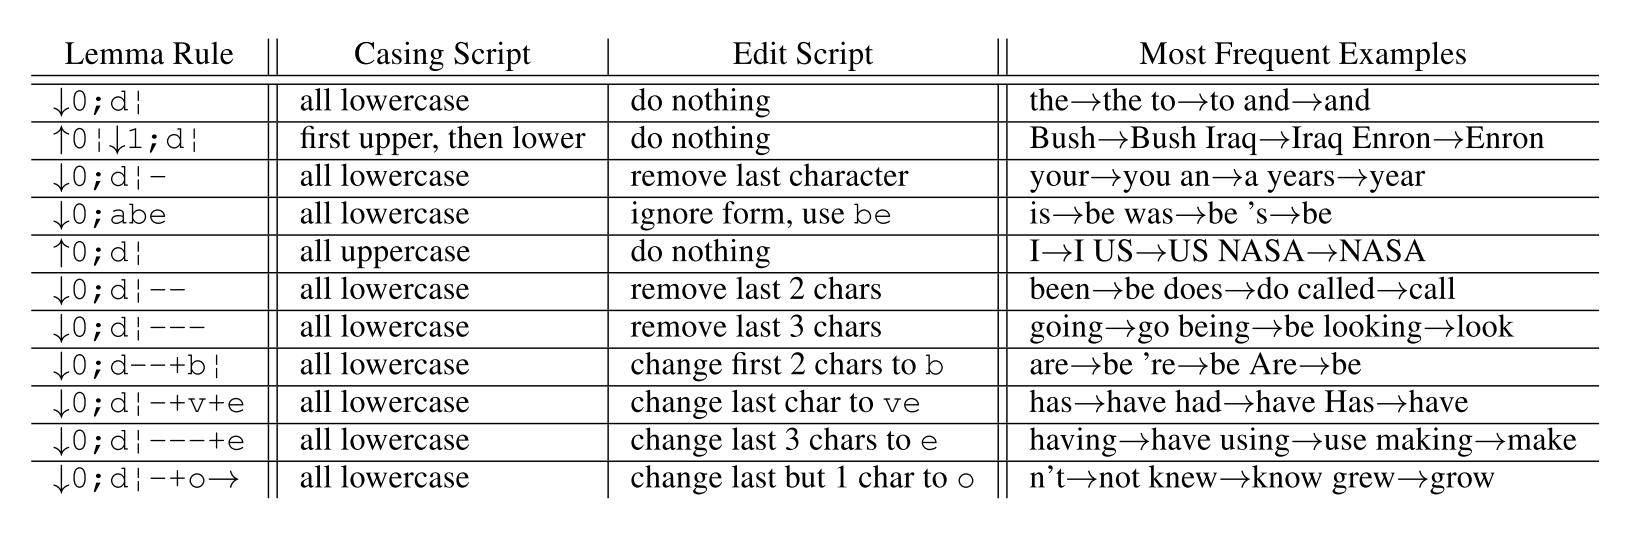
\includegraphics[width=1\textwidth]{../img/lemma_rules}
\protect\caption{
Table 1 from \citep{Straka2019b} presents 10 most common lemma generating rules in English EWT corpus. Each rule has two parts -- casing script for transforming uppercase and lowercase letters, and edit script. Edit script can transform prefix, suffix, or also a root of the word.
}
\label{fig:lemma_rules}
\end{figure}

\begin{table}
\centering
\label{Tab:tagset}
\begin{tabular}{ |c|c|c| } 

 \hline
 Position & Name & Description \\ 
 \hline \hline
 1 & POS & Part of speech \\ \hline
 2 & SubPOS & Detailed part of speech \\ \hline
  3 & Gender & Gender \\ \hline
4 & Number & Number \\\hline
  5 & Case & Case \\ \hline
 6 & PossGender & Possessor's gender \\\hline
  7 & PossNumber & Possessor's number \\ \hline
8 & Person & Person \\\hline
  9 & Tense & Tense \\ \hline
 10 & Grade & Degree of comparison\\\hline
  11 & Negation & Negation \\ \hline
 12 & Voice & Voice \\\hline
 13 & Reserve1 & Reserve \\ \hline
14 & Reserve2 & Reserve \\\hline
  15 & Var & Variant, style \\ 
 \hline

\end{tabular}
\caption{Czech morphology developement is dated from 1989 %TODO zdroj Hajič
and in description of words uses 15-places morphological tags as described in this table taken from \citep{Hana2005}} 
\end{table}

\subsection{Dataset and Preprocessing}
\label{sub:dataset}
Dataset for these tasks is based on Prague Dependency Treebank (PDT) \cite{PDT35}, specifically version 3.5, which is PDT edition from year 2018. Dataset is divided into three parts - train, developement and test.  %TODO jak vypadaji vstupni data - ukazka z tech dat co mam primo!!!
Data consists of sentences with lemmas and tags. For ambiguous words, data contain all possible analysis. For example, Czech word "psa" have one possible lemma ("pes") but two possible tags because it could be one of two possible grammatical cases -- genitive or accusative. Input data for such word looks as follows: \\
\begin{center}
psa pes NNMS2-----A---- NNMS4-----A----
\end{center}, where analysis correspond to 

Input sentences are preprocessed as follows: %TODO mozna az do site? opsat vse z UDPipe2.0 !!!
\begin{itemize}
\item white space deletion
\item mapping characters -- all unknown development and test datasets' characters are then mapped into one \textit{UNK} token. 
\item mapping  words from train into integers -- Simply number from one to number of unique words.
%bertí embeddingy
		%precomputed
		%bert segments ... ke ktere vete a slovu segmenty patri
		%bert subwords .. subwordy - proc subwordy a ze jsou v kontextu a proto musim s vetou celou!!
		%udelat z toho tensor
\end{itemize}

%jaky je preprocessing dat
	%co je analyses?
	%co je lemma rule

	%tedy parsování na slova a věty
	

\subsection{Related Work}
This work aims to improve previously published SOTA results for contextualized embeddings in czech lemmatization and tagging \citep{Straka2019}. 

as described in table \ref{Tab:tagset}.  %TODO a ja pouzivam ty samy? 


%\citep{Horsmann}
%\citep{Plank}
%\citep{Plisson}
%\citep{Straka2019b}
%\citep{Straka2019a}
%\citep{Toutanova2003}
%\citep{Wang2015}
%\citep{Huang2015}
%\citep{Collobert2011} ... preprocessing


\begin{table}[!h]
  \begin{tabular}{|l||c|c|c||c|c|c|}
  \hline
\multirow{2}{*}{Experiment} & \multicolumn{3}{c||}{Without Dictionary}  &
      \multicolumn{3}{c|}{With Dictionary} \\ 
    & Tags & Lemmas & Both & Tags & Lemmas & Both \\ \hline
    StrakaB & 97.94\% & 98.75\% & 97.31\% & 98.05\% & 98.98\% & 97.65\% \\ \hline
    emb (lr 0.0001) &  97.80\% & 98.70\% & 97.17\% & 97.95\% & 98.93\% & 97.55\% \\ \hline
    baseline & 97.04 \% & 98.56 \% & 96.41\% &  97.31  \% & 98.83 \% & 96.90\% \\ \hline 
    StrakaC & 97.67\% & 98.63\% & 97.02\% & 97.91\% & 98.94\% & 97.51\% \\ \hline
  \end{tabular}
  \caption{%TODO cite
  Straka2019B is the best solution from \citep{Straka2019} paper. Straka2019C is a comparable solution  (BERT embeddings only), which was transformed into TF2 in this work.} 
\end{table}

\subsection{Experiments and Architecture}
This chapter describes implemented linguistic models. As mentioned before, this work implements models for three Czech NLP tasks: tagging, lemmatization and sentiment analysis. Common model for first two tasks develops on the paper by \cite[]{straka2019czech} focused on application of contextual embeddings produced by language models as Bert %todo cite
 or Flair. %todo cite. 
 Third task, sentiment analysis, is performed by adding only one fully-connected layer at the top of bert model. So in the opposite to previous tasks, no sophisticated handcrafted pipeline is built and model relies only on the network powers of language structure representation.

The model for this part is build upon a model (and a code) for previous work on Czech NLP processing with contextual embeddings \citep{straka2019czech}. Data preparation %todo trida s odkazem do github
pipeline - tokenization and sentence segmentation is taken over from the paper as well as base structure of lemmatizer and tagger network. 

. Both tasks share one network.

Script allows training of these model variants:
\begin{itemize}
\item baseline model -- original implementation %todo zdroj
of network as described in figure %todo obrazek a zdroj co to dela
\\ \textbf{Embeddings:} %TODO popsat poradne tvar
Model contains potentially embeddings of four types -- pretrained word2vec embeddings %todo zdroj
, word embeddings trained with network, bert embeddings (just in some models as described later) and character-level embeddings.
\item label smoothing -- baseline model with label smoothing %todo zdroj na label smoothing a zdroj na vysvetleni v nektere casti
\item bert embeddings -- model can take precomputed bert embeddings as an input, otherwise embeddings are computed at the beginning and also saved for further use. In this case, data are tokenized by BERT tokenizer. Same principle is used for unknown words as before. Embeddings for word segments are averaged for each original input word, as BERT word segments and sentence words does not correspond to each other one to one. These embeddings serves as additional input to the network as in figure %TODO  %TODO see sectionBert embeddings are contextualized %see section so whole sentence is input into BERT tokenizer.
\item BERT finetunning -- In contrast to the BERT embeddings model, in this case BERT embeddings are also trained during network training, i.e. whole BERT network is chained to baseline network instead of embedding numbers only, gradients are backpropagated throw whole new network and weights are updated also in the BERT part of network.
\end{itemize}
All classification can be done with or without use of a morphological dictionary MorFlex %todo reference
. If the option with dictionary is used, generated tags and lemmas are chosen just from the dictionary. So it is selected lemma and/or tag with maximal likelihood, but just from those presented in the dictionary.

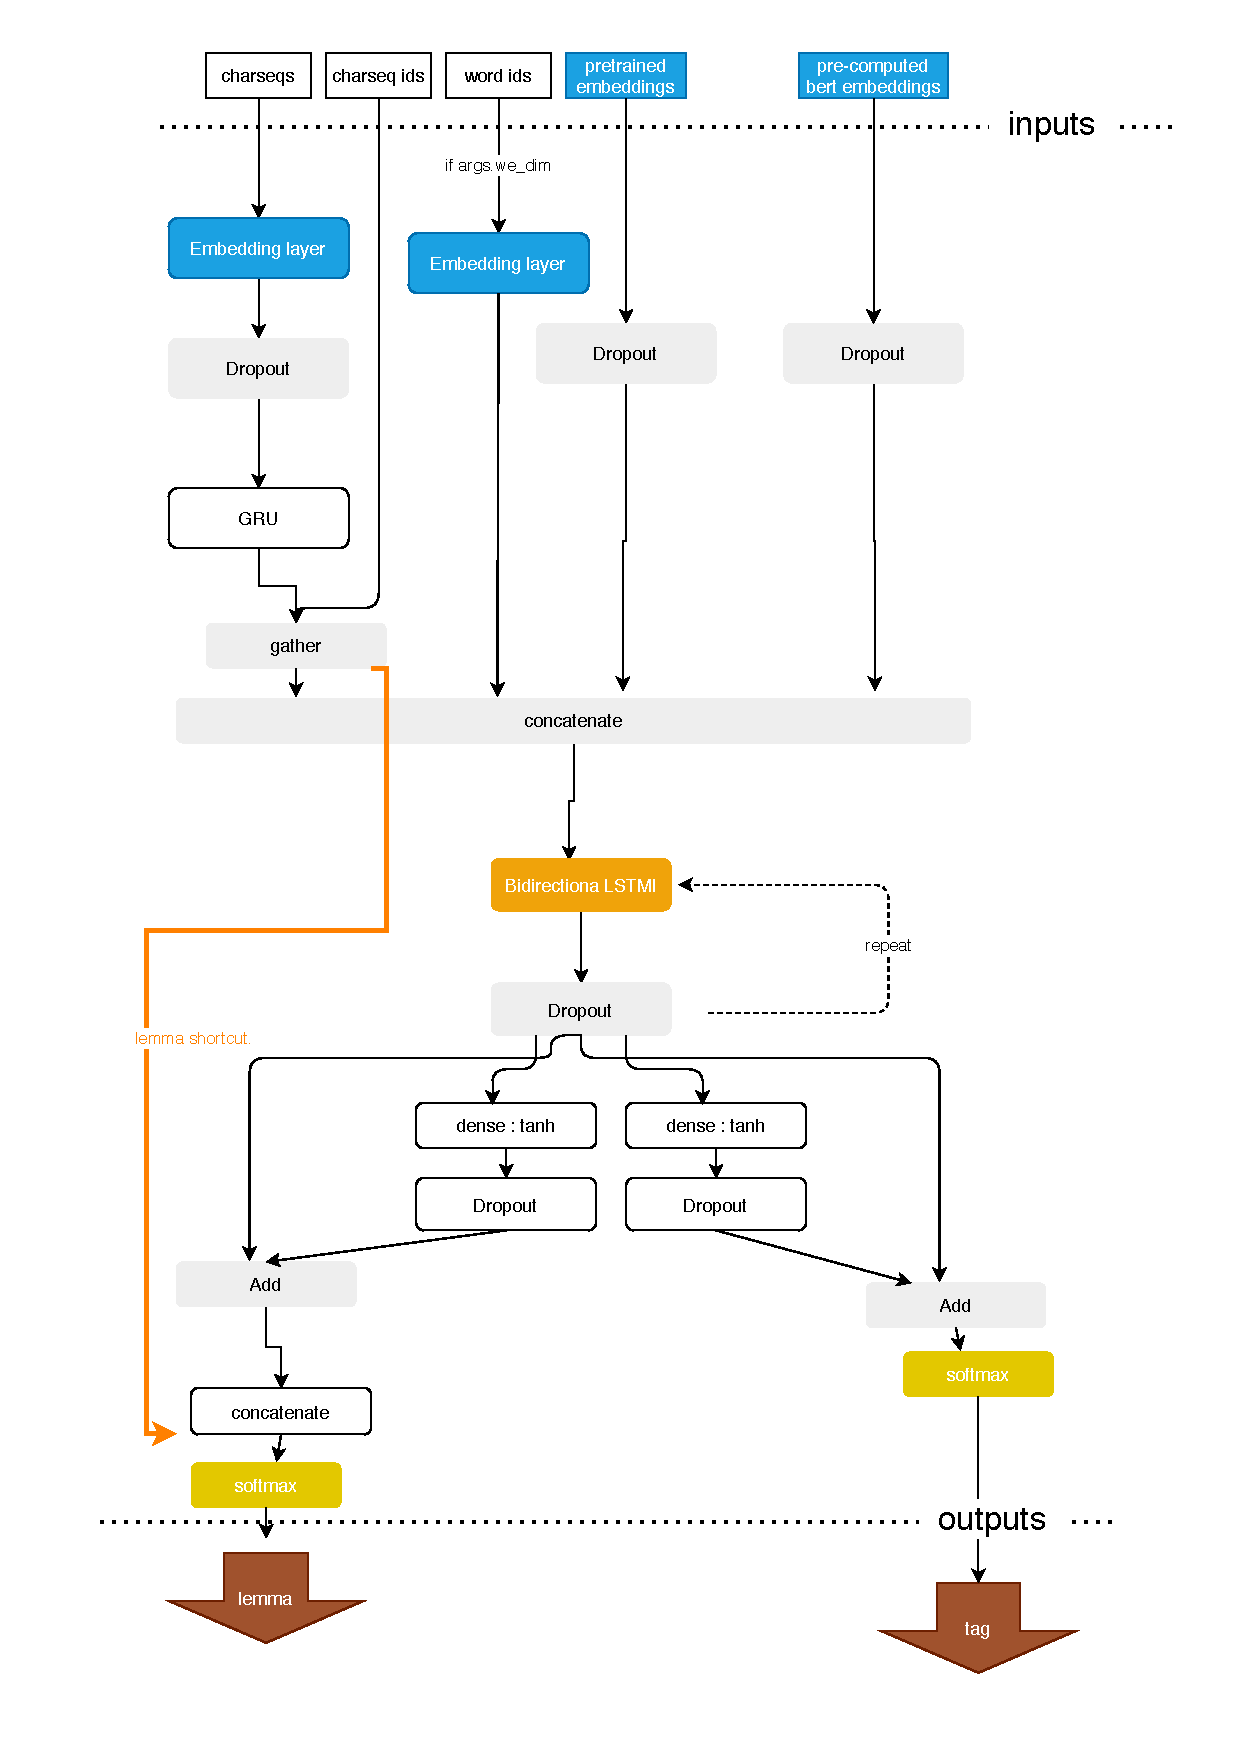
\includegraphics[width=1\columnwidth]{../img/taggermodel.pdf}


\subsection{Results}


